\documentclass[12pt, a4paper]{report}
\usepackage[utf8]{inputenc}
\usepackage{enumitem}
\usepackage{fancyvrb}
\usepackage{minted}
\usepackage{wasysym}

\usepackage[backend=biber,style=alphabetic,sorting=ynt]{biblatex}
\addbibresource{tesina.bib}

\usepackage{graphicx}
\graphicspath{ {./images/} }

\usepackage[pdfpagelabels]{hyperref}
\hypersetup{
    plainpages=false,
    colorlinks=true,
    citecolor=blue,
    linkcolor=blue,
    urlcolor=blue,
    filecolor=magenta,
}

\title{Tesina}
\author{Iñaki Garay}
\date{Septiembre 2020}

\begin{document}

\pagenumbering{Alph}
\begin{titlepage}
\maketitle
\thispagestyle{empty}
\end{titlepage}

\pagenumbering{arabic}
\tableofcontents
\thispagestyle{empty}

\newpage

\addcontentsline{toc}{chapter}{Introducción / Esquema General}
\chapter*{Introducción / Esquema General}

\begin{itemize}[noitemsep]

\item Los compiladores tradicionales tienen una arquitectura de pipeline.

\item Dos requerimientos nuevos paralelos: minimizar tiempo de compilacion y proveer mas informacion de manera mas interactiva a las herramientas de edicion.

\item Los editores y entornos de desarrollo modernos usan LSP (Language Server Protocol). Porque?

\item Una implementacion de LSP require de componentes de compiladores (especialmente analisis).

\item La arquitectura de pipeline no se adapta bien a estos requerimientos modernos de reducir tiempos de compilacion y de proveer informacion online durante edicion.

\item Estos objetivos puede ser logrados mediante compilacion incremental.

\item La compilacion incremental puede ser lograda mediante una arquitectura basada en queries.

\item La arquitectura basada en queries es implementada tomando inspiracion de build systems.

\item Como funciona el sistema de queries de rustc?

\item Rust-analyzer es la segunda implementacion de LSP para rust.

\item Porque no funciono la primera iteracion?

\item Rust-Analyzer usa una libreria, Salsa, para cachear las queries parciales.

\item Como funciona Salsa?

\end{itemize}

\addcontentsline{toc}{chapter}{Motivaciones}
\chapter*{Motivaciones}

Los compiladores ya no son cajas negras que ingestan un conjunto de archivos fuente y producen codigo ensamblador.
De compiladores modernos se espera que:

\begin{itemize}[noitemsep]
\item Sean incrementales, es decir, si se recompila el proyecto despues de producir modificaciones en el código fuente, solo se recompila lo que fue afectado por esas modificaciones.

\item Provean funcionalidad para editores, e.g. saltar a definición, encontrar el tipo de una expresión en una ubicación dada, y mostrar errores al editar.
\end{itemize}

\addcontentsline{toc}{section}{Arquitecturas Tradicionales de Compiladores [Olle20]}
\section*{Arquitecturas Tradicionales de Compiladores [Olle20]}

\noindent
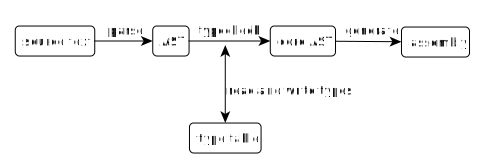
\includegraphics[width=\textwidth]{olle_trad_comp_arq}
\cite{olle_query_based}

Hay muchas variaciones, y frecuentemente mas pasos y representaciones intermedias que las ilustradas, pero la idea esencial es la misma: se empuja codigo fuente por un pipeline y corremos una sequencia fija de transformaciones hasta que finalmente emitimos codigo ensamblador o algun otro lenguaje.
En el camino frecuentemente se necesita leer y actualizar estado interno.
Por ejemplo, se puede actualizar la tabla de tipos durante la fase de verificacion de tipado, para que mas adelante se pueda verificar el tipo de las entidades a las cuales el codigo se refiere.
\cite{olle_query_based}

\addcontentsline{toc}{section}{Language Server Protocol}
\section*{Language Server Protocol}

El Language Server Protocol (LSP) es una protocolo abierto basado en JSON-RPC para el uso entre editores de codigo fuente o entornos de desarrollo integrados (IDE) y servidores que proveen funcionalidades especificas a lenguajes de programacion.
El objetivo del protocolo es permitir que se implemente y distribuya el soporte para un lenguaje de programacion independientemente de un editor o IDE determinado.
Implementar funcionalidad tal como autocompletado, ir a definicion, o mostrar documentacion relacionada a una entidad para un lenguaje de programacion determinado, requieren de esfuerzos significantes.
Tradicionalmente este trabajo se debia repetir para cada herramienta de desarrollo, dado que cada herramienta proveia un API diferente al impl
Un Servidor de Lenguaje provee inteligencia especifica a un lenguaje y se comunica con herramientas de desarrollo mediante un protocolo que permite comunicacion entre procesos.
La idea detras de LSP es estandarizar el protocolo con el cual se comunican los las herramientas de desarrollo y los servidores. De esta manera, un unico servidor de lenguaje puede ser reutilizado por multiples herramientas de desarrollo, las cuales a su vez pueden soportar multiples lenguajes, con esfuerzo minimo.
\cite{language_server_protocol}

Los entornos de desarrollo integrados (IDEs) modernos proveen a desarrolladores funcionalidad sofisticada tale como completado de codigo, refactoreo, navegacion a definicino de un simbolo, resaltamiento de sintaxis, y marcadores de errores y avisos.
Por ejemplo, en un lenguaje basado en texto, un programador podria querer renombra un metodo.
El programador podria o bien manualmente editar los archivos de codigo fuente respectivos y cambiar las ocurrencias apropiadas del nombre viejo del metodo al nuevo, o usar las capacidades para refactorear del IDE para hacer los cambios automaticamente.
Para poder soportar este tipo de refactoreo, un IDE necesita una sofisticado comprehension del lenguaje de programacion en que esta escrito el codigo.
Una herramienta de desarrollo sin ese entendimiento, por ejemplo una que hace una busqueda y reemplazo simple, podria introducir errores.
Por ejemplo, al renombrar un un metodo "read", la herramienta no deberia reemplazar identificadores como "readyState" que contienen el identificador a renombrar, ni tampoco reemplazar porciones de comentarios. Tampoco deberia suceder que renombrar una variable local afecte a variables con nombres similares en otros alcances.
\cite{language_server_protocol_wiki}

Los compiladores e interpretees convencionales son usualmente incapaces de proveer estos servicios de lenguaje, dado que estan implementados con el objetivo de o bien transformar el codigo fuente en codigo objeto o ejecutar inmediatamente el codigo.
Adicionalmente, los servicios de lenguaje deben poder manejar codigo que no esta bien formado, e.g. cuando el programador esta en el medio de editar y no ha terminado de escribir una expresion, procedimiento, u otra construccion del lenguaje.
Mas aun, pequeños cambios que ocurren durante la escritura normalmente cambian la semantica del programa.
Para poder proveer feedback instantaneo al usuario, la herramienta de edicion debe poder evaluar muy rapidamente las consequencias sintacticas y semanticas de una modificacion especifica.
Los compiladores e interpretes, por lo tanto, son pobres candidatos para la produccion de la informacion necesaria para la consumicion por una herramienta de edicion.
\cite{language_server_protocol_wiki}

Previamente al diseño e implementacion de LSP para el desarrollo de Visual Studio Code, la mayoria de los servicios de lenguaje estaban atados a un IDE o editor especifico.
En la ausencia del LSP, los servicios son tipicamente implementados utilizando un API de extension especifica a una herramienta.
Proveer el mismo servicio a otra herramienta de edicion requiere de un esfuerzo para adaptar el codigo existente para que el servicio pueda soportar las interfaces de la segunda herramienta.
\cite{language_server_protocol_wiki}

\noindent
\includegraphics[width=0.9\textwidth]{lsp}

LSP permite desacoplar los servicios de lenguaje del editor de tal manera que los servicios se pueden contener en un servidor de lenguaje de proposito general.
Cual editor puede acceder a soporte sofisticado para muchos lenguajes diferentes al hacer uso de los servidores de lenguaje existentes.
Similarmente, un programador involucrado en el desarrollo de un lenguaje nuevo puede crear servicios para ese lenguaje y hacerlo inmediatamente disponible para editores existentes.
Hacer uso de servidores de lenguaje a traves del LSP por lo tanto tambien reduce la carga sobre los desarrolladores de herramientas de edicion, dado que no necesitan desarrollar sus propios servicios de lenguaje para cada lenguaje que quieren soportar.
El LSP tambien habilita la distribucion y desarrollo de servidores contribuidos por terceros, tales como usuarios finales, sin participacion ni por parte de los desarrolladores del compilador del lenguaje o por los desarrolladores de la herramienta de edicion para la cual se esta agregando soporte de lenguaje.
\cite{language_server_protocol_wiki}

LSP no se limita a lenguajes de programacion.
Puede ser utilizacion para cualquier lenguaje basado en texto, tales como lenguajes de especificacion o especificos a dominions (DSL).
\cite{language_server_protocol_wiki}

\addcontentsline{toc}{section}{Velocidad de Compilación}
\section*{Velocidad de Compilación}

Mejorar los tiempos de compilacion ha sido un foco principal despues de que Rust llego a la version 1.0.
Sin embargo, gran parte del trabajo en pos de este objetivo ha sido sentar las bases arquitectonicas dentro del compilador.

Uno de los proyectos que esta construyendo sobre esta base, y que deberia mejorar los tiempos de compilacion para flujos de trabajo tipicos es la compilacion incremental.
La compilacion incremental evita repetir trabajo cuando se compila un paquete, lo cual llevara en ultima instancia a un ciclo de edicion-compilacion-debug mas rapido.
\cite{rust_blog_incremental_compilation}

\addcontentsline{toc}{chapter}{Mecanismos}
\chapter*{Mecanismos}

\addcontentsline{toc}{section}{Compilación Incremental}
\section*{Compilación Incremental}

La compilación incremental es una forma de computación incremental aplicada a la compilación.
En contraste con compiladores comúnes que realizan "builds limpios" y ante un cambio en el código fuente recompilan todas las unidades de compilación, un compilador incremental solo recompila las unidades modificadas.
Al construir sobre el trabajo hecho previamente, el compilador incremental evita la ineficiencia de repetir trabajo ya realizado.
Se puede decir que un compilador incremental reduce la granularidad de las unidades de compilación tradicionales a la vez que mantiene la semántica del lenguaje.
\cite{wiki_incremental_compiler}

Muchas herramientas de desarrollo aprovechan compiladores incrementales para proveer a sus usuarios un entorno mucho mas interactivo.
No es inusual que un compilador incremental sea invocado por cada cambio en un archivo fuente, de tal manera que el usuario es informado inmediatamente de cualquier error de compilación causado por sus modificaciones.
Este esquema, en contraste con el modelo de compilación tradicional, acorta el ciclo de desarrollo considerablemente.
\cite{wiki_incremental_compiler}

Una desventaja de este esquema es que el compilador no puede optimizar fácilmente el código que compila, dada la localidad y el alcance reducido de los cambios.
Normalmente esto no es un problema, dado que la optimización del código generado se aplica solamente al producir un \textit{release build}, instancia en la cual se puede usar el compilador tradicional.
\cite{wiki_incremental_compiler}

\addcontentsline{toc}{section}{Arquitectura Basada en Queries [Olle20]}
\section*{Arquitectura Basada en Queries [Olle20]}

\addcontentsline{toc}{subsection}{Pasar de pipelines a queries [Olle20]}
\subsection*{Pasar de pipelines a queries [Olle20]}

Que se necesita para obtener el tipo de un identificador calificado?
En una arquitectura basada en pipelines, se buscaria el tipo en la tabla de simbolos.
Con queries, hay que pensarlo de manera distinta.
En lugar de depender de haber actualizado un fragmento de estado, se computa de cero.
En una primera iteracion, se hace siempre completamente de cero.
Primero se averigua de cual archivo viene el nombre, y luego se leen el contenido del archivo, se parsea, posiblemente se realize algo de resolucion de nombres para saber a que nombres se refiere el codigo dado lo que se importa, y por ultimo se busca la definicion cuyo nombre ha sido resuelto y se verifica su tipo, finalmente retornandolo.

\textit{We first find out what file the name comes from, then read the contents of the file, parse it, perhaps we do name resolution to find out what the names in the code refer to given what is imported, and last we look up the name-resolved definition and type check it, returning its type.}

\begin{minted}{haskell}
fetchType :: QualifiedName -> IO Type
fetchType (QualifiedName moduleName name) = do
    fileName <- moduleFileName moduleName
    sourceCode <- readFile fileName
    parsedModule <- parseModule sourceCode
    resolvedModule <- resolveNames parsedModule
    let definition = lookup name resolvedModule
    inferDefinitionType definition
\end{minted}

Refactoreando este esquema en funcionas mas chicas.

\begin{minted}{haskell}
fetchParsedModule :: ModuleName -> IO ParsedModule
fetchParsedModule moduleName = do
  fileName <- moduleFileName moduleName
  sourceCode <- readFile fileName
  parseModule moduleName

fetchResolvedModule :: ModuleName -> IO ResolvedModule
fetchResolvedModule moduleName = do
  parsedModule <- fetchParsedModule moduleName
  resolveNames parsedModule

fetchType :: QualifiedName -> IO Type
fetchType (QualifiedName moduleName name) = do
  resolvedModule <- fetchResolvedModule moduleName
  let definition = lookup name resolvedModule
  inferDefinitionType definition
\end{minted}

Notemos que cada una de estas funciones hace todo de cero, i.e. cada una realiza un prefijo cada vez mas largo del trabajo total que se haria en un pipeline.
Esto ha resultado ser un patron comun en compiladores basados en queries.
Una forma de mejorar la eficiencia de este esquema es agregar una capa de memoizacion alrededor de cada funcion.
De esta manera, se ejecuta trabajo copmutacionalmente demandante la primera vez que se invoca una funcion con un argumento dado, pero las llamadas subsiguientes son mas baratas porque pueden devolver el resultado cacheado.
Esto es la esencia la arquitectura basadas en queries, pero en lugar de usar un cache por funcion, se utiliza un cache central, indexado por query.
\cite{olle_query_based}

\addcontentsline{toc}{section}{Why Incremental Compilation in the First Place? [Woe16]}
\section*{Why Incremental Compilation in the First Place? [Woe16]}

Gran parte del tiempo de un programador se pasa en el ciclo de trabajo editar-compilar-debuguear:

\begin{itemize}
\item se realiza un pequeño cambio (frecuentemente en un unico modulo o funcion),
\item se corre el compilador para convertir el codigo en un objeto ejecutable,
\item se ejecuta el programa resultante o un conjunto de pruebas unitarias para ver el resultado del cambio.
\end{itemize}

Despues de eso, se vuelve al primer paso, realizar otro pequeño cambio informado por el conocimiento adquirido en la iteracion previa.
Este bucle de alimentacion esencial es el nucleo de la actividad diaria de un programador.
Se busca que el tiempo que se pasa detenido mientras se espera que el compilador produzca el compilador ejecutable sea lo mas breve posible.

La compilacion incremental es una forma de aprovechar el hecho que poco cambia entre compilaciones durante el flujo de trabajo normal.
Muchos, si no la mayoria, de los cambios entre sesiones de compilacion solo tienen un impacto local en el codigo maquina del binario producido, mientras que la mayor parte del programa, al igual que a nivel codigo, termina igual, bit a bit.
La compilacion incremental apunta a retener la mayor parte posible de estas partes sin cambios a la vez que se rehace solo la cantidad de trabajo que debe hacerse.
\cite{rust_blog_incremental_compilation}

\addcontentsline{toc}{section}{How Do You Make Something "Incremental"? [Woe16]}
\section*{How Do You Make Something "Incremental"? [Woe16}

Ya se detallo que computar algo incrementalmente significa actualizar solo aquellas partes de la salida de la computacion que necesita ser adaptada en respuesta a los cambios dados en las entradas de la computacion.
Una estrategia basica que podemos emplear para lograr esto es ver una computacion grande (tal como compilar un programa completo) como una composicion de muchas computaciones pequeñas interrelacionadas que construyen una sobre otra.
Cada una de estas computaciones mas pequeñas producira un resultado intermedio que puede ser cacheado y reutilizado en una iteracion subsiguiente, evitando la necesidad de re-computar ese resultado intermedio en particular.
\cite{rust_blog_incremental_compilation}

\addcontentsline{toc}{section}{An Incremental Compiler [Woe16]}
\section*{An Incremental Compiler [Woe16]}

La forma en que se eligio implementar la incrementalidad en el compilador de Rust es directa: una sesion de compilacion incremental sigue exactamente los mismos pasos que una sesion de compilacion batch.
Sin embargo, cuando el flujo de control llegue a un punto en el cual esta a punto de computar un resulto intermedio no trivial, intentara cargar ese resultado del cache de compilacion incremental en disco en su lugar.
Si existe una entrada valida en el cache, el copmilador puede saltear la computacion de ese dato en particular.
Este es un esquema (simplificado) de de las diferentes fases de compilacion y los resultados intermedios que producen:
\cite{rust_blog_incremental_compilation}

\noindent
\includegraphics[width=0.9\textwidth]{woe16_compiler_phases}

Primero, el compilador parse el codigo fuente en un arbol de sintaxis abstracto (AST).
El AST pasa luego a la fase de analisis que produce informacion de tipos y el MIR para cada funcion.
Luego de eso, si el analisis no encontro ningun error, la fase de generacion de codigo transformara la version MIR del programa en su version de codigo maquina, emitiendo un archivo objeto por cada modulo de codigo.
En la ultima fase todos los archivo objeto son linkeados juntos en el binario final, que puede ser una libreria o un ejecutable.
Hasta ahora las cosas parecen bastante simples: en lugar de computar algo por segunda vez, sencillamente cargar el valor desde el cache.
Las cosas se complican cuando es necesario saber si es efectivamente valido usar un valor del cache o si hay que recomputarlo porque alguna entrada ha cambiado.
\cite{rust_blog_incremental_compilation}

\addcontentsline{toc}{section}{Seguimiento de Dependencias [Olle20]}
\section*{Seguimiento de Dependencias [Olle20]}

El seguimiento, o \textit{tracking}, de dependencias, es provista por librerias tales como Rock, Shake, o Salsa.
Estas librerias proveen parte de la funcionalidad necesaria para crear compiladores basados en queries.

Rock es una libreria experimental fuertemente inspirada por Shake y el paper \textit{Build systems à la carte} \cite{mokhov2018build}.
Esencialmente implementa un framework de sistema de construccion \textit{build system framework}, como \texttt{make}.
Los sistemas de construccion tienen mucho en comun con compiladores modernos dado que tambien queremos que sean incrementales, i.e. que aprovechen los resultados de construcciones anteriores al construir uno nuevo con pocos cambios.
Sin embargo, tambien tienen una diferencia: a la mayoria de los sistemas de construccion no les importa el tipo de sus queries dado que trabajan sobre archivos y sistema de archivos.
El esquema detallado en \textit{Build systems à la carte} se aproxima mejor a lo necesario en el caso de un compilador.
En esta publicacion detallan un sistema en el cual el usuario escribe un conjunto de computaciones, tareas, que toman una clave y retornan un valor, y elige un tipo adecuado para las claves y otro para los valores.
Las tareas se formulan asumiendo que van a ser ejecutadas en un entorno en el cual existe una funcion \texttt{fetch} de tipo \texttt{Key -> Task[Value]}, donde \texttt{Task} es un tipo que describe las reglas del sistema de construccion, la cuale puede ser usada para obtener los valores de una dependencia con una clave dada.
El sistema de construccion tiene control sobre que codigo corre al momento de ejecutar \texttt{fetch}, de tal manera que se puede variar la granularidad del seguimiento de dependencias, memoisacion, y actualizaciones incrementales.
\textit{Build systems à la carte} tambien explora que tipo de sistemas de construccion obtenemos cuando variamos lo que puede realizar una tarea \textit{Task}, e.g. si es una monada o un aplicativo.
Un problema que surge inmediatamente es que no hay ningun tipo satisfactorio para \texttt{Value}.
E.g. puede haber una query para obtener el modulo donde esta definido un tipo, y otra para obtener la representacion del tipo dado el nombre calificado de un tipo.
\cite{olle_query_based}

% \addcontentsline{toc}{section}{Indexed queries [Olle20]}
% \section*{Indexed queries [Olle20]}
%
% - Rock allows us to index the key type by the return type of
% the query. The Key type in our running example becomes the
% following GADT:
%
% \begin{minted}{haskell}
% data Key a where
%   ParsedModuleKey :: ModuleName -> Key ParsedModule
%   ResolvedModuleKey :: ModuleName -> Key ResolvedModule
%   TypeKey :: QualifiedName -> Key Type
% \end{minted}
%
% - The fetch function gets the type forall a. Key a -> Task
% a, so we get a ParsedModule when we run fetch
% (ParsedModuleKey "Data.List"), like we wanted, because the
% return type depends on the key we use.
%
% - Now that we know what fetch should look like, it's also
% worth revealing what the Task type looks like in Rock, more
% concretely.
%
% - As mentioned, it's a thin layer around IO, providing a way
% to fetch keys (like Key above):
%
% - The rules of our compiler, i.e. its "Makefile", then
% becomes the following function, reusing the functions from
% above:
% \cite{olle_query_based}
%
% \begin{minted}{haskell}
% rules :: Key a -> Task a
% rules key = case key of
%   ParsedModuleKey moduleName ->
%     fetchParsedModule moduleName
%   ResolvedModuleKey moduleName ->
%     fetchResolvedModule moduleName
%   TypeKey qualifiedName ->
%     fetchType qualifiedName
% \end{minted}
% \cite{olle_query_based}

\addcontentsline{toc}{section}{Caching [Olle20]}
\section*{Caching [Olle20]}


\begin{verbatim}
- The most basic way to run a Task in Rock is to directly
call the rules function when a Task fetches a key.

- This results in an inefficient build system that
recomputes every query from scratch.

- But the Rock library lets us layer more functionality onto
our rules function, and one thing that we can add is
memoisation.

- If we do that Rock caches the result of each fetched key
by storing the key-value pairs of already performed fetches
in a dependent hashmap.

- This way, we perform each query at most once during a
single run of the compiler.
\end{verbatim}
\cite{olle_query_based}

\addcontentsline{toc}{section}{Verifying dependencies and reusing state [Olle20]}
\section*{Verifying dependencies and reusing state [Olle20]}

\begin{verbatim}
- Another kind of functionality that can be layered onto the
rules function is incremental updates. When it's used, Rock
keeps track of what dependencies a task used when it was
executed (much like Shake) in a table, i.e. what keys it
fetched and what the values were.

- Using this information it's able to determine when it's
safe to reuse the cache from a previous run of the compiler
even though there might be changes in other parts of the
dependency graph.

- This fine-grained dependency tracking also allows reusing
the cache when a dependency of a task changes in a way that
has no effect.

- For example, whitespace changes might trigger a re-parse,
but since the AST is the same, the cache can be reused in
queries that depend on the parse result.
\end{verbatim}
\cite{olle_query_based}

\addcontentsline{toc}{section}{Reverse dependency tracking [Olle20]}
\section*{Reverse dependency tracking [Olle20]}

\begin{verbatim}
- Verifying dependencies can be too slow for real-time
tooling like language servers, because large parts of the
dependency graph have to be traversed just to check that
most of it is unchanged even for tiny changes.

- For example, if we make changes to a source file with many
large imports, we need to walk the dependency trees of all
of the imports just to update the editor state for that
single file.

- This is because dependency verification by itself needs to
go all the way to the root queries for all the dependencies
of a given query, which can often be a large proportion of
the whole dependency tree.

- To fix this, Rock can also be made to track reverse
dependencies between queries.

- When e.g. a language server detects that a single file has
changed, the reverse dependency tree is used to invalidate
the cache just for the queries that depend on that file by
walking the reverse dependencies starting from the changed
file.

- Since the imported modules don't depend on that file, they
don't need to be re-checked, resulting in much snappier
tooling!
\end{verbatim}
\cite{olle_query_based}

\addcontentsline{toc}{chapter}{Caso de Estudio: Rustc}
\chapter*{Caso de Estudio: Rustc}

Rustc, el compilador de rust, tiene su propia implementacion de queries.

\addcontentsline{toc}{section}{Rustc Dependency graphs [Woe16]}
\section*{Rustc Dependency graphs [Woe16]}

Existe un modelo formal que puede usarse para modelar los resultados intermedios de una computacion y su propiedad de estar actualizad de una manera directa: los grafos de dependencias.
Cada entrada y cada resultado intermedio son representados como un nodo en un grafo dirigido.
Los arcos en el grafo representan cual resultado intermedio o entrada puede tener influencia en otro resultado intermedio.
En general los arboles

\begin{verbatim}
- There is a formal method that can be used to model a
computation's intermediate results and their individual
"up-to-dateness" in a straightforward way: dependency
graphs.

- It looks like this: Each input and each intermediate
result is represented as a node in a directed graph. The
edges in the graph, on the other hand, represent which
intermediate result or input can have an influence on some
other intermediate result.

- Note, by the way, that the above graph is a tree just
because the computation it models has the form of a tree. In
general, dependency graphs are directed acyclic graphs

- What makes this data structure really useful is that we
can ask it questions of the form "if X has changed, is Y
still up-to-date?". We just take the node representing Y and
collect all the inputs Y depends on by transitively
following all edges originating from Y. If any of those
inputs has changed, the value we have cached for Y cannot be
relied on anymore.
\end{verbatim}
\cite{rust_blog_incremental_compilation}

\addcontentsline{toc}{section}{Dependency Tracking in the Compiler [Woe16]}
\section*{Dependency Tracking in the Compiler [Woe16]}

\noindent
\includegraphics[width=0.9\textwidth]{woe16_compiler_dep_graph}

\noindent
\includegraphics[width=0.9\textwidth]{woe16_compiler_cache_purge}

\begin{verbatim}
- When compiling in incremental mode, we always build the
dependency graph of the produced data: every time, some
piece of data is written (like an object file), we record
which other pieces of data we are accessing while doing so.

- The emphasis is on recording here. At any point in time
the compiler keeps track of which piece of data it is
currently working on (it does so in the background in
thread-local memory).

- This is the currently active node of the dependency graph.
Conversely, the data that needs to be read to compute the
value of the active node is also tracked: it usually already
resides in some kind container (e.g. a hash table) that
requires invoking a lookup method to access a specific
entry.

- We make good use of this fact by making these lookup
methods transparently create edges in the dependency graph:
whenever an entry is accessed, we know that it is being read
and we know what it is being read for (the currently active
node).

- This gives us both ends of the dependency edge and we can
simply add it to the graph. At the end of the compilation
sessions we have all our data nicely linked up, mostly
automatically.

- This dependency graph is then stored in the incremental
compilation cache directory along with the cache entries it
describes.

- At the beginning of a subsequent compilation session, we
detect which inputs (=AST nodes) have changed by comparing
them to the previous version. Given the graph and the set of
changed inputs, we can easily find all cache entries that
are not up-to-date anymore and just remove them from the
cache.

- Anything that has survived this cache validation phase can
safely be re-used during the current compilation session.

- There are a few benefits to the automated dependency
tracking approach we are employing. Since it is built into
the compiler's internal APIs, it will stay up-to-date with
changes to the compiler, and it is hard to accidentally
forget about. And if one still forgets using it correctly
(e.g. by not declaring the correct active node in some
place) then the result is an overly conservative, but still
"correct" dependency graph: It will negatively impact the
re-use ratio but it will not lead to incorrectly re-using
some outdated piece of data.

- Another aspect is that the system does not try to predict
or compute what the dependency graph is going to look like,
it just keeps track. A large part of our (yet to be written)
regression tests, on the other hand, will give a description
of what the dependency graph for a given program ought to
look like. This makes sure that the actual graph and the
reference graph are arrived at via different methods,
reducing the risk that both the compiler and the test case
agree on the same, yet wrong, value.
\end{verbatim}
\cite{rust_blog_incremental_compilation}

\begin{verbatim}
- Let's take a look at some of the implications of what
  we've learned so far:
  - The dependency graph reflects the actual dependencies
    between parts of the source code and parts of the output
    binary.
  - If there is some input node that is reachable from many
    intermediate results, e.g. a central data type that is
    used in almost every function, then changing the
    definition of that data type will mean that everything
    has to be compiled from scratch, there's no way around
    it.
- In other words, the effectiveness of incremental
  compilation is very sensitive to the structure of the
  program being compiled and the change being made.
  Changing a single character in the source code might very
  well invalidate the whole incremental compilation cache.
  Usually though, this kind of change is a rare case and
  most of the time only a small portion of the program has
  to be recompiled.
\end{verbatim}
\cite{rust_blog_incremental_compilation}

\addcontentsline{toc}{section}{The Current Status of the Implementation [Woe16]}
\section*{The Current Status of the Implementation [Woe16]}

El estado actual de rustc a fines de 2019.
Para la primera implementacion de compilacion incremental, implementada a principios de 2019, el equipo de rustc de focalizo en cachear archivos objeto.
Consequentemente, si esta fase se puede saltear aunque sea para parte de un codigo, se puede lograr el mayor impacto en tiempos de compilacion.
Con esto en mente, tambien se puede estimar la cota superior de cuanto tiempo se puede ahorrar: si el compilador pasa N segundos optimizando cuando compila un crate, entonces la compilacion incremental puede reducir los tiempos de compilado en a lo sumo esos N segundos.
Otra area que tiene una gran influencia en la efectividad de la primera implementacion de es la granularidad del seguimiento de dependencias.
Depende de la implementacion cuan fina es la granularidad de los grafos de dependencias, y la implementacion actual es media gruesa.
Por ejemplo, el grafo de dependencias solo tiene un unico nodo para todos los metodos en un \texttt{impl} (bloque de implementacion de un trait).
En consecuencia, el compilador considerara que cambiaron todos los metodos de ese \texttt{impl} aunque solo haya cambiado uno solo.
Esto por supuesto significa que mas codigo sera recompilado de lo que seria estrictamente necesario.
\cite{rust_blog_incremental_compilation}

\addcontentsline{toc}{chapter}{Caso de Estudio: Rust-analyzer y Salsa}
\chapter*{Caso de Estudio: Rust-analyzer y Salsa}

Rust-Analyzer utiliza una libreria llamada salsa.

\addcontentsline{toc}{section}{Como funciona salsa?}
\section*{Como funciona salsa?}

La idea central de salsa es definir el programa como un conjunto de \textit{queries}.
Cada query se usa como una función $K \to V$ que mapea de una clave de tipo $K$ a un valor de tipo $V$.

Las queries en salsa son de dos variedades basicas:
\begin{itemize}[noitemsep]
\item \textbf{Entradas:}
definen los inputs basicos al sistema, los cuales pueden cambiar en cualquier momento.
\item \textbf{Funciones:}
funciones puras (sin efectos secundarios) que transforman las entradas en otros valores.
Los resultados de estas queries se memoizan para evitar recomputarlas.
Cuando se modifican las entradas, salsa determina cuales valores memoizados pueden ser reutilizados y cuales deben ser recomputados.
\end{itemize}

El esquema general de utilizacion de salsa consiste en tres pasos:

\begin{enumerate}[noitemsep]
\item Definir uno o mas grupos de queries que contendran las entradas y las queries requeridas.
Se puede definir mas de un grupo para separar las queries en componentes.
\item Definir las queries.
\item Definir la base de datos, la cual contendra el almacenamiento para las entradas y queries utilizadas.
\end{enumerate}

\addcontentsline{toc}{chapter}{Conclusiones}
\chapter*{Conclusiones}

La mayoria de los lenguajes modernos necesitan tener una estrategia en cuanto a la provision de herramientas de desarrollo, y la construccion de compiladores en base a sistemas de queries parace ser un acercamiento con mucha promesa.
Con queries el desarrollador del compilador no necesita manejar explicitamente la actualizacion e invalidacion de un conjunto de caches ad hoc, lo cual puede ser el resultado cuando se agregan actualizaciones incrementales a una arquitectura de compilador tradicional en pipeline.
En un sistema basado en queries se maneja el estado incremental de manera centralizada, reduciendo la posibilidad de errores.
Las queries son excelentes para las herramientas porque permiten pedir por el valor de cualquier query en cualquier momento sin tener que preocuparse sobre el orden o efectos temporales, al igual que con un Makefile bien escrito.
El sistema copmutara o recuperar valores cacheads por la query y sus dependencias automaticamente de una manera incremental.
Los compialdores basados en queries son ademas sorprendentemente facil de paralelizar.
Dado que se puede ejecutar cualquier query en cualquier momento, y se memoizan la primera vez que corren, se pueden disparar varias queries en paralelo sin preocuparse demasiado.
\cite{olle_query_based}

Planes futuros para rustc (09/2019)

Los dos ejes principales a lo largo de los cuales se buscara mejorar la eficiencia de rustc son:
\begin{itemize}[noitemsep]
\item Cachear mas resultados intermediosm como MIR e informacion de tipo, permitiendo que el compilador evite repetir mas y mas pasos.
\item Mejorar la precision del seguimiento de dependencias, para que el compilador encuentre menos falsos positivos durante la invalidacion del cache.
\end{itemize}
\cite{rust_blog_incremental_compilation}

\addcontentsline{toc}{chapter}{Source Notes}
\chapter*{Source Notes}

\addcontentsline{toc}{section}{Anders Hejlsberg on Modern Compiler Construction}
\section*{Anders Hejlsberg on Modern Compiler Construction}
\cite{hejlsberg_modern_compiler_construction}

\addcontentsline{toc}{section}{Build Systems a la Carte}
\section*{Build Systems a la Carte}
\cite{mokhov2018build}

\addcontentsline{toc}{section}{How Salsa Works}
\section*{How Salsa Works (2019.01)}
\cite{niko2019salsaworks}

\addcontentsline{toc}{section}{Salsa In More Depth}
\section*{Salsa In More Depth (2019.01)}
\cite{niko2019salsadepth}

\addcontentsline{toc}{section}{Fuentes}
\section*{Fuentes}

\begin{itemize}[noitemsep]

\item General
  \begin{itemize}[noitemsep]
  \item \href{https://www.youtube.com/watch?v=wSdV1M7n4gQ}{\CheckedBox Youtube: Anders Hejlsberg on Modern Compiler Construction} \cite{hejlsberg_modern_compiler_construction}
  \item \href{https://en.wikipedia.org/wiki/Incremental_compiler}{\CheckedBox Wikipedia: Incremental Compiler} \cite{wiki_incremental_compiler}
  \item \href{https://ollef.github.io/blog/posts/query-based-compilers.html}{\CheckedBox Olle Fredriksson: Query-based compiler architectures} \cite{olle_query_based}
  \item \href{https://blog.rust-lang.org/2016/09/08/incremental.html}{\CheckedBox Rust Blog: Incremental Compilation} \cite{rust_blog_incremental_compilation}
  \item \href{https://www.microsoft.com/en-us/research/publication/build-systems-la-carte/}{\Square Build Systems A La Carte} \cite{mokhov2018build}
  \item \href{https://www.youtube.com/watch?v=b_T-eCToX1I}{\CheckedBox Youtube: 2016 LLVM Developers’ Meeting: D. Dunbar “A New Architecture for Building Software”} \cite{dunbar2016}
  \end{itemize}

\item Rustc Dev Guide
  \begin{itemize}[noitemsep]
  \item \href{https://rustc-dev-guide.rust-lang.org/overview.html}{\Square Overview of the Compiler}
  \item \href{https://rustc-dev-guide.rust-lang.org/compiler-src.html}{\Square High-level overview of the compiler source}
  \item \href{https://rustc-dev-guide.rust-lang.org/query.html}{\Square Queries: demand-driven compilation}
    \begin{itemize}[noitemsep]
    \item \href{https://rustc-dev-guide.rust-lang.org/queries/query-evaluation-model-in-detail.html}{\Square The Query Evaluation Model in Detail}
    \item \href{https://rustc-dev-guide.rust-lang.org/queries/incremental-compilation.html}{\Square Incremental compilation}
    \item \href{https://rustc-dev-guide.rust-lang.org/queries/incremental-compilation-in-detail.html}{\Square Incremental Compilation In Detail}
    \item \href{https://rustc-dev-guide.rust-lang.org/incrcomp-debugging.html}{\Square Debugging and Testing Dependencies}
    \item \href{https://rustc-dev-guide.rust-lang.org/queries/profiling.html}{\Square Profiling Queries}
    \item \href{https://rustc-dev-guide.rust-lang.org/salsa.html}{\Square How Salsa works}
    \end{itemize}
  \end{itemize}

\item Rust Analyzer
  \begin{itemize}[noitemsep]
  \item \href{https://rust-analyzer.github.io/}{\Square Rust Analyzer}
  \item \href{https://rust-analyzer.github.io/manual.html}{\Square Manual}
  \item \href{https://rust-analyzer.github.io/blog}{\Square Blog}
  \item \href{https://github.com/rust-analyzer/rust-analyzer/tree/master/docs/dev}{\Square rust-analyzer/tree/master/docs/dev}
  \item \href{https://ferrous-systems.com/blog/rust-analyzer-2019/}{\Square Rust Analyzer in 2018 and 2019}
  \item \href{https://ferrous-systems.com/blog/rust-analyzer-status-opencollective/}{\Square Status of rust-analyzer}
  \item \href{https://blog.logrocket.com/intro-to-rust-analyzer/}{\Square 2020 Intro to Rust Analyzer}
  \item \href{https://dev.to/bnjjj/what-i-learned-contributing-to-rust-analyzer-4c7e}{\Square 2020 What I learned contributing to Rust-Analyzer}
  \item \href{https://www.youtube.com/watch?v=7_7ckOKZCJE}{\Square Youtube: Are we *actually* IDE yet? A look on the Rust IDE Story - Igor Matuszewski}
  \item \href{https://www.youtube.com/watch?v=ANKBNiSWyfc}{\Square Youtube: Rust analyzer guide}
  \item \href{https://www.youtube.com/watch?v=DGAuLWdCCAI}{\Square Youtube: rust analyzer syntax trees}
  \item \href{https://www.youtube.com/watch?v=Lmp3P9WNL8o}{\Square Youtube: rust-analyzer type-checker overview by flodiebold}
  \item \href{https://www.youtube.com/playlist?list=PLXajQV_H-DxLMBt0amcuxgTeOTj6L-YGl}{\Square Youtube: Rust Analyzer Q\&A}
  \end{itemize}

\item Salsa
  \begin{itemize}[noitemsep]
  \item \href{https://salsa-rs.github.io/salsa/}{\Square The Salsa Book}
  \item \href{https://www.youtube.com/playlist?list=PL85XCvVPmGQh0P_VEPVM2ZIlBwl4MQMNY}{\Square Youtube: Incremental Compilation Working Group}
  \item \href{https://www.youtube.com/watch?v=N6b44kMS6OM}{\Square Youtube: Responsive compilers - Nicholas Matsakis - PLISS 2019}
  \item \href{https://www.youtube.com/watch?v=LIYkT3p5gTs}{\CheckedBox Youtube: Things I Learned (TIL) - Nicholas Matsakis - PLISS 2019}
  \item \href{https://www.youtube.com/watch?v=_muY4HjSqVw}{\Square Youtube: How Salsa Works (2019.01)}
  \item \href{https://www.youtube.com/watch?v=i_IhACacPRY}{\Square Youtube: Salsa In More Depth (2019.01)}
  \item \href{https://www.youtube.com/watch?v=Xr-rBqLr-G4}{\Square Youtube: RLS 2.0, Salsa, and Name Resolution}
  \end{itemize}

\item Rust Compilation Speed
  \begin{itemize}[noitemsep]
  \item \href{https://vfoley.xyz/rust-compile-speed-tips/}{\Square How to alleviate the pain of Rust compile times}
  \item \href{https://blog.mozilla.org/nnethercote/2016/10/14/how-to-speed-up-the-rust-compiler/}{\Square Nethercote: How to speed up the Rust compiler}
  \item \href{https://blog.mozilla.org/nnethercote/2016/11/23/how-to-speed-up-the-rust-compiler-some-more/}{\Square Nethercote: How to speed up the Rust compiler some more}
  \item \href{https://blog.mozilla.org/nnethercote/2018/04/30/how-to-speed-up-the-rust-compiler-in-2018/}{\Square Nethercote: How to speed up the Rust compiler in 2018}
  \item \href{https://blog.mozilla.org/nnethercote/2018/06/05/how-to-speed-up-the-rust-compiler-some-more-in-2018/}{\Square Nethercote: How to speed up the Rust compiler some more in 2018}
  \item \href{https://blog.mozilla.org/nnethercote/2018/11/06/how-to-speed-up-the-rust-compiler-in-2018-nll-edition/}{\Square Nethercote: How to speed up the Rust compiler in 2018: NLL edition}
  \item \href{https://blog.mozilla.org/nnethercote/2018/05/17/the-rust-compiler-is-getting-faster/}{\Square Nethercote: The Rust compiler is getting faster}
  \item \href{https://blog.mozilla.org/nnethercote/2019/07/25/the-rust-compiler-is-still-getting-faster/}{\Square Nethercote: The Rust compiler is still getting faster}
  \item \href{https://blog.mozilla.org/nnethercote/2019/07/17/how-to-speed-up-the-rust-compiler-in-2019/}{\Square Nethercote: How to speed up the Rust compiler in 2019}
  \item \href{https://blog.mozilla.org/nnethercote/2019/10/11/how-to-speed-up-the-rust-compiler-some-more-in-2019/}{\Square Nethercote: How to speed up the Rust compiler some more in 2019}
  \item \href{https://blog.mozilla.org/nnethercote/2019/12/11/how-to-speed-up-the-rust-compiler-one-last-time-in-2019/}{\Square Nethercote: How to speed up the Rust compiler one last time in 2019}
  \item \href{https://blog.mozilla.org/nnethercote/2020/04/24/how-to-speed-up-the-rust-compiler-in-2020/}{\Square Nethercote: How to speed up the Rust compiler in 2020}
  \item \href{https://blog.mozilla.org/nnethercote/2020/08/05/how-to-speed-up-the-rust-compiler-some-more-in-2020/}{\Square Nethercote: How to speed up the Rust compiler some more in 2020}
  \item \href{https://blog.mozilla.org/nnethercote/2020/09/08/how-to-speed-up-the-rust-compiler-one-last-time/}{\Square Nethercote: How to speed up the Rust compiler one last time}
  \item \href{https://pingcap.com/blog/rust-compilation-model-calamity}{\Square PingCAP Blog: The Rust Compilation Model Calamity}
  \item \href{https://pingcap.com/blog/generics-and-compile-time-in-rust}{\Square PingCAP Blog: Generics and Compile-Time in Rust}
  \item \href{https://pingcap.com/blog/rust-huge-compilation-units}{\Square PingCAP Blog: Rust's Huge Compilation Units}
  \item \href{https://pingcap.com/blog/reasons-rust-compiles-slowly}{\Square PingCAP Blog: A Few More Reasons Rust Compiles Slowly}
  \end{itemize}

\item Miscellaneous
  \begin{itemize}[noitemsep]
  \item \href{https://www.youtube.com/watch?v=S2dK5lLFD_0}{\Square Youtube: Making Fast Incremental Compiler for Huge Codebase - Michał Bartkowiak - code::dive 2019}
  \item \href{https://www.youtube.com/watch?v=JbS8a-Ba0Ck}{\Square Youtube: Starting with Semantics - Sylvan Clebsch - PLISS 2019}
  \item \href{https://www.youtube.com/watch?v=mt6pIpt5Wk0}{\Square Youtube: Polyhedral Compilation as a Design Pattern for Compilers (1/2) - Albert Cohen - PLISS 2019}
  \item \href{https://www.youtube.com/watch?v=3TNT5rFVTUY}{\Square Youtube: Polyhedral Compilation as a Design Pattern for Compilers (2/2) - Albert Cohen - PLISS 2019}
  \item \href{https://www.youtube.com/watch?v=yvlhwZgUPG0}{\Square Youtube: First-Class Continuations: What and Why - Arjun Guha}
  \item \href{https://www.youtube.com/watch?v=n_GhkL8GDAk}{\Square Youtube: Implementing First-Class Continuations by Source to Source Translation - Arjun Guha - PLISS 2019}
  \item \href{https://www.youtube.com/watch?v=Lr4cMmaJHrg}{\Square Youtube: Static Program Analysis (part 1/2) - Anders Møller - PLISS 2019}
  \item \href{https://www.youtube.com/watch?v=6QQSIIvH-F0}{\Square Youtube: Static Program Analysis (part 2/2) - Anders Møller - PLISS 2019}
  \end{itemize}

\end{itemize}

\printbibliography[
  heading=bibintoc,
  title={Bibliografia}
]

\end{document}
